% SIX-PAGE IEEE version (MLNLP 2026), condensed from ieee/main.tex on 2026-10-18.
% ieee/main.tex is the full version and is unchanged; submit it as supplementary material.
% Tables, figure and bibliography are SHARED with ../paper, so every number here comes from
% the same generated macros as both full versions. Do not type a result in by hand.
\documentclass[conference]{IEEEtran}
\usepackage[numbers]{natbib}
\usepackage[T1]{fontenc}
\usepackage[utf8]{inputenc}
\usepackage{microtype}
\usepackage{booktabs}
\usepackage{graphicx}
\usepackage{amsmath}
\usepackage{xspace}
\xspaceaddexceptions{\%}
\usepackage{url}
\usepackage[hidelinks]{hyperref}
% GENERATED by scripts/make_h8_tables.py -- do not hand-edit
\newcommand{\hEightOrderings}{3\xspace}
\newcommand{\hEightItems}{500\xspace}
\newcommand{\hEightWorstRange}{2.0\xspace}
\newcommand{\hEightWorstSD}{1.10\xspace}
\newcommand{\hEightBFCells}{8\xspace}
\newcommand{\hEightBFZero}{8\xspace}
\newcommand{\hEightRepFloor}{0.000\xspace}
\newcommand{\hEightNCells}{15\xspace}
\newcommand{\hEightPinned}{2\xspace}
\newcommand{\hEightFrozenB}{32\xspace}
\newcommand{\hEightEngine}{1.0.0\xspace}
\newcommand{\hEightSDOrderings}{10\xspace}
\newcommand{\hEightWorstSDTen}{1.14\xspace}
\newcommand{\hEightRangeTen}{3.8\xspace}
\newcommand{\hEightBFTenZero}{2\xspace}
\newcommand{\hEightBFTenCells}{2\xspace}
\newcommand{\hEightSDLevel}{64\xspace}

% GENERATED by scripts/make_h8_tables.py -- do not hand-edit
\newcommand{\hEightSpotGPU}{A10G\xspace}
\newcommand{\hEightSpotItems}{500\xspace}
\newcommand{\hEightSpotOrderings}{10\xspace}
\newcommand{\hEightSpotLevel}{32\xspace}
\newcommand{\hEightSpotBFText}{0.0\xspace}
\newcommand{\hEightSpotText}{69.8\xspace}
\newcommand{\hEightTenText}{71.2\xspace}
\newcommand{\hEightSpotSD}{0.70\xspace}
\newcommand{\hEightTenSD}{0.87\xspace}
\newcommand{\hEightSpotFloor}{8\xspace}
\newcommand{\hEightSpotMarlinOn}{53.4\xspace}
\newcommand{\hEightSpotMarlinOff}{0.0\xspace}

% GENERATED by scripts/make_figures.py -- do not hand-edit
\newcommand{\hOneItems}{12,600\xspace}
\newcommand{\hOneCapBfOne}{15.2\xspace}
\newcommand{\hOneCapBfFour}{0.5\xspace}
\newcommand{\hOneCapGptqOne}{22.2\xspace}
\newcommand{\hOneCapGptqFour}{2.0\xspace}
\newcommand{\hOneCapAwqOne}{29.5\xspace}
\newcommand{\hOneCapAwqFour}{5.7\xspace}
\newcommand{\hOneDiscardGptq}{415\xspace}
\newcommand{\hOneDiscardBf}{215\xspace}
\newcommand{\hOnePMin}{0.048\xspace}
\newcommand{\hOneAlphaMin}{0.0125\xspace}
\newcommand{\hOneBestEst}{-1.80\xspace}
\newcommand{\hOneBestCI}{-3.60 to -0.02\xspace}
\newcommand{\hOneLenBf}{169\xspace}
\newcommand{\hOneLenGptq}{173\xspace}
\newcommand{\hOneLenAwq}{180\xspace}

% GENERATED by scripts/analyze_h6.py -- do not hand-edit
\newcommand{\hSixQwenGptq}{-13.2\xspace}
\newcommand{\hSixQwenGptqCI}{-16.6 to -10.0\xspace}
\newcommand{\hSixQwenAwq}{-8.4\xspace}
\newcommand{\hSixMaxOther}{1.8\xspace}
\newcommand{\hSixRejected}{2\xspace}
\newcommand{\hSixM}{6\xspace}
\newcommand{\hSixQwenBfGen}{67.6\xspace}
\newcommand{\hSixQwenBfLL}{80.2\xspace}
\newcommand{\hSixQwenGptqGen}{74.4\xspace}
\newcommand{\hSixQwenGptqLL}{73.8\xspace}
\newcommand{\hSixItems}{500\xspace}

% GENERATED by scripts/make_h3_tables.py -- do not hand-edit
\newcommand{\hThreeRows}{12\xspace}
\newcommand{\hThreeRecords}{105,950\xspace}
\newcommand{\hThreeArcGptqEight}{+0.00\xspace}
\newcommand{\hThreeArcGptqEightLo}{-0.51\xspace}
\newcommand{\hThreeArcGptqEightHi}{+0.51\xspace}
\newcommand{\hThreeArcGptqFour}{+0.00\xspace}
\newcommand{\hThreeArcGptqFourLo}{-0.51\xspace}
\newcommand{\hThreeArcGptqFourHi}{+0.51\xspace}
\newcommand{\hThreeArcAwq}{+0.00\xspace}
\newcommand{\hThreeArcAwqLo}{-0.51\xspace}
\newcommand{\hThreeArcAwqHi}{+0.51\xspace}
\newcommand{\hThreeArcNfFour}{+0.00\xspace}
\newcommand{\hThreeArcNfFourLo}{-0.51\xspace}
\newcommand{\hThreeArcNfFourHi}{+0.51\xspace}
\newcommand{\hThreeBbhGptqEight}{+0.06\xspace}
\newcommand{\hThreeBbhGptqEightLo}{-0.67\xspace}
\newcommand{\hThreeBbhGptqEightHi}{+0.76\xspace}
\newcommand{\hThreeBbhGptqFour}{+1.73\xspace}
\newcommand{\hThreeBbhGptqFourLo}{+0.79\xspace}
\newcommand{\hThreeBbhGptqFourHi}{+2.70\xspace}
\newcommand{\hThreeBbhAwq}{+1.55\xspace}
\newcommand{\hThreeBbhAwqLo}{+0.61\xspace}
\newcommand{\hThreeBbhAwqHi}{+2.52\xspace}
\newcommand{\hThreeBbhNfFour}{-0.97\xspace}
\newcommand{\hThreeBbhNfFourLo}{-1.91\xspace}
\newcommand{\hThreeBbhNfFourHi}{-0.06\xspace}
\newcommand{\hThreeGsmGptqEight}{+0.53\xspace}
\newcommand{\hThreeGsmGptqEightLo}{-0.33\xspace}
\newcommand{\hThreeGsmGptqEightHi}{+1.42\xspace}
\newcommand{\hThreeGsmGptqFour}{-5.21\xspace}
\newcommand{\hThreeGsmGptqFourLo}{-6.77\xspace}
\newcommand{\hThreeGsmGptqFourHi}{-3.61\xspace}
\newcommand{\hThreeGsmAwq}{-0.91\xspace}
\newcommand{\hThreeGsmAwqLo}{-2.50\xspace}
\newcommand{\hThreeGsmAwqHi}{+0.66\xspace}
\newcommand{\hThreeGsmNfFour}{-8.44\xspace}
\newcommand{\hThreeGsmNfFourLo}{-9.91\xspace}
\newcommand{\hThreeGsmNfFourHi}{-6.95\xspace}
\newcommand{\hThreeArcBound}{0.51\xspace}
\newcommand{\hThreeArcN}{1,500\xspace}
\newcommand{\hThreeExcludesNull}{5\xspace}
\newcommand{\hThreeHolmM}{8\xspace}
\newcommand{\hThreeHetTasks}{+6.93\xspace}
\newcommand{\hThreeHetTasksLo}{+5.09\xspace}
\newcommand{\hThreeHetTasksHi}{+8.76\xspace}
\newcommand{\hThreeHetArms}{-4.30\xspace}
\newcommand{\hThreeHetArmsLo}{-5.84\xspace}
\newcommand{\hThreeHetArmsHi}{-2.75\xspace}
\newcommand{\hThreeGsmDemoExcluded}{gsm8k\xspace}
\newcommand{\hThreeGsmDemoGptqEight}{+0.05\xspace}
\newcommand{\hThreeGsmDemoGptqFour}{-13.12\xspace}
\newcommand{\hThreeGsmDemoAwq}{-7.91\xspace}
\newcommand{\hThreeGsmDemoNfFour}{-4.68\xspace}

% GENERATED by scripts/make_h4_tables.py -- do not hand-edit
\newcommand{\hFourEffects}{108\xspace}
\newcommand{\hFourExcludesNull}{48\xspace}
\newcommand{\hFourRung}{strict\xspace}
\newcommand{\hFourChurnTask}{BBH\xspace}
\newcommand{\hFourChurnArm}{GPTQ W4A16\xspace}
\newcommand{\hFourChurnLost}{423\xspace}
\newcommand{\hFourChurnGained}{421\xspace}
\newcommand{\hFourChurnTotal}{844\xspace}
\newcommand{\hFourChurnNet}{-0.06\xspace}
\newcommand{\hFourGainTask}{ARC-C\xspace}
\newcommand{\hFourGainArm}{AWQ W4A16\xspace}
\newcommand{\hFourGainNet}{+2.73\xspace}
\newcommand{\hFourLossTask}{GSM8K\textsubscript{CoT}\xspace}
\newcommand{\hFourLossArm}{bnb NF4\xspace}
\newcommand{\hFourLossNet}{-9.88\xspace}
\newcommand{\hFourStratumCells}{27\xspace}
\newcommand{\hFourStratumBelowHalf}{14\xspace}


\title{Reproducibility Failures in Quantized Model Evaluation:\\
Item Ordering Moves 4-Bit Accuracy and Leaves \texttt{bf16} Exactly Unchanged}

\author{%
\IEEEauthorblockN{Joseph Sankoorikal Johny}
\IEEEauthorblockA{Independent Researcher\\Seattle, USA\\\texttt{joseph.sankoorikal@gmail.com}}
\and
\IEEEauthorblockN{Syed Ahmed Danish}
\IEEEauthorblockA{Independent Researcher\\Hartford, USA\\\texttt{syed.danish47@gmail.com}}
\and
\IEEEauthorblockN{Aniruddha Sharma}
\IEEEauthorblockA{Independent Researcher\\Seattle, USA\\\texttt{anirudh217sharma@gmail.com}}}

\begin{document}
\maketitle

\begin{abstract}
A reported quantization cost is one score minus another, so any part of the evaluation that
penalises the two models unequally ends up inside the reported gap. We evaluate three
instruction-tuned models at five precisions with the engine, decoding and prompts fixed,
and vary properties of the evaluation that protocols do not report. Two results are
established by intervention or by a pre-registered contrast that survives multiple-comparison
correction. First, item submission order changes 4-bit accuracy by up to
\hEightWorstSDTen{} points of standard deviation across \hEightSDOrderings{} orderings and
leaves \texttt{bf16} \emph{exactly} unchanged, with the engine's batch-invariant mode
enabled: that mode does not cover the quantized matrix-multiply kernels, and disabling them
removes the variation for GPTQ and AWQ. The GPTQ result replicates on a second GPU
architecture. Second, the extraction rule changes the measured quantization effect with a
task-dependent sign, moving GPTQ W4A16 relative to \texttt{bf16} by \hThreeBbhGptqFour{}
points on BBH and by \hThreeGsmGptqFour{} on GSM8K, so no single correction restores
comparability. Supporting results bound the picture, and we give remedies with measured
costs, a released corpus of 105{,}950 generations and a runnable order-invariance probe.
\end{abstract}

\begin{IEEEkeywords}
quantization, reproducibility, LLM evaluation, inference kernels, batch invariance
\end{IEEEkeywords}

\section{Introduction}
\label{sec:intro}

When a paper reports that 4-bit quantization costs two points of accuracy, that number was
not measured. It is the difference between two measurements, and anything about the
evaluation that penalises the two runs unequally lands in the reported gap.
\citet{kurtic2025bf16} showed that reported degradation had been overstated and traced the
excess to untuned quantization-side hyperparameters. Our concern is the residual that
survives that tuning, and our mechanisms act on the evaluation, not on the quantized model.

\emph{Changing every score is not the same as changing the gap between scores.} Lenient
answer extraction is known to raise absolute scores \citep{jo2025finding,yu2025xfinder}, and
prompt formatting moves them substantially \citep{sclar2024formatspread}. A choice that
lowers every model's score equally is a nuisance, because the gap survives it. A choice that
lowers some models' scores more than others changes the gap, and so contaminates every
published comparison that did not report it. We test for the second kind, and find it.

\emph{Two headline results.} Varying only the order in which the same items are submitted
changes 4-bit accuracy by up to \hEightWorstSDTen{} points of standard deviation and leaves
\texttt{bf16} exactly unchanged, because the engine's batch-invariant mode does not cover
the quantized kernels it selects by default; disabling them removes the variation
(\S\ref{sec:h8}). And the extraction rule interacts with precision with a sign that depends
on the task, so no single correction recovers comparability (\S\ref{sec:h3}).

\emph{This is not an argument for scoring more permissively.} \citet{ren2026shortcut} find
that 8.2--44.1\% of answers graded correct are reached by shortcut hacking, and we find that
lenient extraction also destroys some correct answers. The goal is to \emph{calibrate}
extraction, not to loosen it. Nor is it an argument that quantization is benign: benchmarks
also \emph{understate} quantization damage relative to human judgement
\citep{marchisio2024multilingual,dutta2024accuracy}. Both directions hold at once, because
they are different quantities.

\emph{Contributions.} (i) Item ordering moves 4-bit accuracy and leaves \texttt{bf16} exactly
unchanged, with the mechanism pinned by intervention to kernels the batch-invariant mode does
not cover, and replicated on a second GPU architecture. (ii) The precision-by-scoring
interaction changes sign across tasks and differs across methods. (iii) Supporting results:
a cross-process reproducibility failure, a bounded null for the generation budget, and a
log-likelihood control on ARC. (iv) Remedies with measured costs, and three fields every
protocol should report. (v) A released corpus of 105{,}950 generations and an
order-invariance probe.

\section{Related Work}
\label{sec:related}

\citet{pape2026silent} is the nearest prior work. They survey 35{,}000 publications, find that
only 36\% of papers without released code name even their inference backend, and show that
switching backend alone moves GSM8K by 16.6 points; \citet{masoudian2026sideeffect} attribute
roughly 39\% of out-of-the-box variance to the serving configuration. But their controlled
comparison runs at \emph{batch size one}, chosen to prevent batching-induced instability, at
FP16. The instability they design out is the one we study: we fix the engine, weights and
decoding, vary only which items share a batch, and attribute the divergence to a named
quantized kernel.

\citet{he2025nondeterminism} traced nondeterministic inference to reductions whose order
depends on how many requests share a batch, and introduced the batch-invariant kernels that
vLLM's batch-invariant mode builds on. We show that its guarantee does not extend to the
4-bit GPTQ and AWQ kernels vLLM selects by default. \citet{hua2025flaw} ask whether prompt
sensitivity is a model property or an evaluation artifact; we vary the scorer rather than the
prompt. Whether quantization lengthens chain-of-thought is disputed
\citep{lian2026inflates,lotfi2026longer,liu2025quantization}, and no study on either side
sweeps the generation cap. \citet{kurt2026which} report strict-versus-flexible GSM8K gaps of
41 to 64 points across \texttt{llama.cpp} quantizations without interpreting them.

\section{Method}
\label{sec:method}

\emph{Design.} Three instruction-tuned models (Qwen2.5-3B, Phi-3.5-mini, Llama-3.1-8B), each
pinned by commit, at five precisions: \texttt{bf16}, GPTQ-8bit, GPTQ-4bit, AWQ-4bit and
bitsandbytes NF4. Tasks are GSM8K with chain-of-thought, BIG-Bench Hard and ARC-Challenge,
evaluated with the lm-evaluation-harness \citep{biderman2024lessons}. Every manipulation is
one factor at a time from a single fixed reference condition.

\emph{Quantization.} GPTQ and AWQ are produced by one tool at one normalised calibration
budget (512 sequences of up to 2048 tokens from \texttt{ultrachat\_200k}), identical for
every arm and model, because the tool's own examples differ by 8$\times$ in budget between
the two methods. Group size is 128, and activation reordering is explicitly disabled to match
the vendors' released checkpoints. NF4 is quantized in flight at load.

\emph{Scoring.} Every generation is stored once and scored by a ladder of extractors, or
\emph{rungs}, on the same text, so the ladder costs no extra generation: \emph{strict}, the
harness's canonical regular expression; \emph{strict-last}, the same expression taking the last
match; \emph{permissive}, the harness's flexible extractor; \emph{symbolic} equivalence; and a
trained judge \citep{chen2025xverify} that we did not validate and on which no claim rests. The
headline contrast is strict against permissive, both deterministic and auditable. We validated
both against 250 human labels from two annotators (raw agreement 0.975, Gwet's AC1 0.968).
Auditing our own pipeline found that a rule we had added ahead of the harness's returned worse
answers on 2{,}068 of 105{,}950 generations, which our unit tests never caught. Repairing it
changed the conclusion of two interaction estimates and the sign of one; all numbers here are
after the repair.

\emph{Compliance and truncation.} Every generation records the engine's termination reason and
its token count, which cannot be reconstructed later, so a wrong answer can be split into one
the model did not know, one it knew but did not state in the expected form, and one cut off by
the budget. We also separate an answer being \emph{extractable} from the model having
\emph{committed} to it, because a fallback that takes the last number in a truncated trace
extracts something the model never asserted.

\emph{Serving.} One engine (vLLM \hEightEngine), greedy decoding, every sampling field pinned,
batch-invariant mode on \citep{he2025nondeterminism}, tensor parallelism of one, prefix
caching off, and a maximum of \hEightFrozenB{} co-resident sequences. That value was measured
rather than assumed: it is the largest at which every arm is bitwise reproducible across
repeated identical runs, and any arm less reproducible than \texttt{bf16} sets a noise floor
below which we claim no effect. The full configuration,
rubric and pre-registration are in the supplementary material.

\section{Results}
\label{sec:results}

The first two subsections are the headline results, established by intervention
(\S\ref{sec:h8}) or by a pre-registered contrast that survives Holm--Bonferroni
(\S\ref{sec:h3}). The third collects supporting results.

\subsection{Item ordering moves 4-bit accuracy and leaves \texttt{bf16} unchanged}
\label{sec:h8}

Requests are batched dynamically, so an item's position decides which other items share its
batch, and so the order in which the engine sums intermediate results. Floating-point
addition is not associative, and in chain-of-thought generation one differing token changes
every token after it. Running the same items again in the \emph{same} order changes nothing:
none of the \hEightNCells{} model-and-precision combinations produced a single differing
output. Every difference below is caused by the ordering.

\begin{table}[t]
\centering
\caption{Accuracy across \hEightSDOrderings{} orderings of the same \hEightItems{} items
(Qwen2.5-3B, L40S, $B=\hEightSDLevel$), in accuracy points. The standard deviation is the
inferential quantity; the range grows with the number of orderings.}
\label{tab:h8-sd}
\small
% GENERATED by scripts/make_h8_tables.py -- do not hand-edit
\begin{tabular}{lcccc}
\toprule
& \multicolumn{2}{c}{strict} & \multicolumn{2}{c}{permissive} \\
\cmidrule(lr){2-3}\cmidrule(lr){4-5}
arm & SD & range & SD & range \\
\midrule
\textsc{bf16} & 0.00 & 0.00 & 0.00 & 0.00 \\
GPTQ W4A16 & 1.00 & 3.20 & 0.67 & 2.40 \\
AWQ W4A16 & 0.80 & 2.60 & 1.14 & 3.80 \\
bnb NF4 & 0.06 & 0.20 & 0.06 & 0.20 \\
\bottomrule
\end{tabular}

\end{table}

\emph{Accuracy moves, and only for quantized arms.} Under all \hEightSDOrderings{} orderings,
\texttt{bf16} accuracy is identical at both rungs (Table~\ref{tab:h8-sd}). Every quantized arm
moves, by up to \hEightWorstSDTen{} points of standard deviation and a range of up to
\hEightRangeTen{}. The shift is deterministic given an ordering, so repeated runs cannot
average it away, and it moves accuracy in both directions, so no ordering is the correct one.
We report the standard deviation rather than the spread because the spread grows with effort:
the same quantity over three orderings gave a spread of 1.6 points, and over
\hEightSDOrderings{} gives \hEightRangeTen{}, with no change to the underlying effect.

\begin{table}[t]
\centering
\caption{Paired intervention at $B=8$: the same inputs and engine with and without the Marlin
and Machete kernels. Text divergence in percent, accuracy SD in points.}
\label{tab:h8-mechanism}
\small
% GENERATED by scripts/make_h8_tables.py -- do not hand-edit
\begin{tabular}{lcccc}
\toprule
& \multicolumn{2}{c}{text divergence} & \multicolumn{2}{c}{accuracy SD} \\
\cmidrule(lr){2-3}\cmidrule(lr){4-5}
arm & Marlin on & off & Marlin on & off \\
\midrule
GPTQ W4A16 & 53.2 & 0.0 & 0.42 & 0.00 \\
AWQ W4A16 & 53.6 & 0.0 & 0.35 & 0.00 \\
bnb NF4 & 49.4 & 49.4 & 0.31 & 0.31 \\
\bottomrule
\end{tabular}

\end{table}

\emph{The batch-invariant mode does not cover Marlin or Machete.} Disabling those two kernels
through \texttt{VLLM\_DISABLED\_KERNELS}, and changing nothing else, drives divergence to zero
for GPTQ and AWQ, on text and on accuracy (Table~\ref{tab:h8-mechanism}). Both of our
checkpoints use the \texttt{compressed-tensors} format, which vLLM loads through a 4-bit
kernel chooser with no batch-invariance check, in 0.26.0 and in the source of 0.32.0, the
newest release in October 2026; it selects Marlin whether or not the mode is on. The source
shows four such gaps: that chooser, the AutoGPTQ loader, the sampler, and kernel autotuning.
The only guard we found, which avoids Marlin in this mode, is in the loader for AutoAWQ-format
checkpoints, a path ours never take. NF4 never
used these kernels and is unchanged by the intervention, so its ordering sensitivity has a
second, separate cause. The intervention locates the mechanism; it does not explain the
arithmetic, and we do not identify which reduction differs.

\emph{The effect replicates on a second GPU architecture.} On an NVIDIA \hEightSpotGPU{}
(Ampere, SM 8.6) with the same image, engine, weights and probe, \texttt{bf16} text differs on
\hEightSpotBFText\% of items across \hEightSpotOrderings{} orderings. GPTQ W4A16 text differs
on \hEightSpotText\% (\hEightTenText\% on the L40S), with a strict accuracy SD of
\hEightSpotSD{} (\hEightTenSD{} on the L40S), and disabling Marlin and Machete takes it from
\hEightSpotMarlinOn\% to \hEightSpotMarlinOff\%.

\subsection{The scoring rule changes the measured quantization effect, unevenly}
\label{sec:h3}

For each arm we take the strict-to-permissive gain in accuracy and subtract \texttt{bf16}'s
gain on the same items, bootstrapped over item clusters. Positive means leniency helps the
quantized arm more than \texttt{bf16}.

\begin{table*}[t]
\centering
\caption{Precision $\times$ scoring interaction in accuracy points against \texttt{bf16}, on
\hThreeRecords{} generations. \textbf{Bold} excludes the null. $\dagger$: ARC-C is exactly
zero, so the interval is the Wilson zero-event bound.}
\label{tab:h3-interaction}
\small
% GENERATED by scripts/make_h3_tables.py -- do not hand-edit
\begin{tabular}{lrcrcrc}
\toprule
& \multicolumn{2}{c}{ARC-C (gen.) ($n$=1,500)} & \multicolumn{2}{c}{BBH ($n$=3,300)} & \multicolumn{2}{c}{GSM8K\textsubscript{CoT} ($n$=3,957)} \\
\cmidrule(lr){2-7}
arm & est. & 95\% CI & est. & 95\% CI & est. & 95\% CI \\
\midrule
GPTQ W8A16 & +0.00$^{\dagger}$ & [-0.51, +0.51] & +0.06 & [-0.67, +0.76] & +0.53 & [-0.33, +1.42] \\
GPTQ W4A16 & +0.00$^{\dagger}$ & [-0.51, +0.51] & \textbf{+1.73} & [+0.79, +2.70] & \textbf{-5.21} & [-6.77, -3.61] \\
AWQ W4A16 & +0.00$^{\dagger}$ & [-0.51, +0.51] & \textbf{+1.55} & [+0.61, +2.52] & -0.91 & [-2.50, +0.66] \\
bnb NF4 & +0.00$^{\dagger}$ & [-0.51, +0.51] & \textbf{-0.97} & [-1.91, -0.06] & \textbf{-8.44} & [-9.91, -6.95] \\
\bottomrule
\end{tabular}

\end{table*}

\emph{The interaction is real, and its sign depends on the task.} \hThreeExcludesNull{} of
the \hThreeHolmM{} BBH and GSM8K estimates survive Holm--Bonferroni
(Table~\ref{tab:h3-interaction}). On BBH, leniency helps the 4-bit arms more than
\texttt{bf16}: GPTQ W4A16 \hThreeBbhGptqFour{}~pp and AWQ W4A16 \hThreeBbhAwq{}~pp. On
GSM8K\textsubscript{CoT} it reverses: GPTQ W4A16 \hThreeGsmGptqFour{}~pp and NF4
\hThreeGsmNfFour{}~pp.

\emph{The disagreement is tested, not observed.} Two contrasts were pre-registered and named
structurally before either was computed. Holding the arm fixed and varying the task gives
\hThreeHetTasks{}~pp $[\hThreeHetTasksLo, \hThreeHetTasksHi]$; holding the task fixed and
comparing GPTQ with AWQ at matched bit width gives \hThreeHetArms{}~pp
$[\hThreeHetArmsLo, \hThreeHetArmsHi]$. Both reject under Holm--Bonferroni. A uniform
interaction would have a remedy, one offset. A heterogeneous one does not: the correction that
fits GPTQ on BBH has the wrong sign on GSM8K, so the extraction rule has to be reported.

GPTQ W8A16 is null on both generative tasks, as a dose-response predicts, and ARC-C is exactly
zero for every arm, bounded within $\pm\hThreeArcBound$~pp at $n$=\hThreeArcN. GSM8K under the
hash-marker prompt is excluded from the family, because instruction-tuned models rarely emit
the \texttt{\#\#\#\#} marker unprompted and strict extraction there measures marker
compliance; its estimates are large and negative (GPTQ W4A16 \hThreeGsmDemoGptqFour{}~pp, AWQ
W4A16 \hThreeGsmDemoAwq{}~pp), and we show them only as the extreme of that gradient.

\subsection{Supporting results}
\label{sec:supporting}

\emph{Reproducibility holds within a process and fails across processes.} Within one process,
generation is bitwise reproducible: zero differing items across 42{,}380 paired comparisons.
Across processes, the same configuration diverges on up to 45\% of items for one model. A
practitioner who repeats a measurement in one process therefore concludes the pipeline is
deterministic, using exactly the check a careful person would run. We refuted four causes
(KV-cache sizing, memory-driven batching, weight provenance and sampling defaults) and do not
identify the real one.

\emph{A fixed generation budget truncates quantized outputs more often, at a bounded accuracy
cost.} We ran \hOneItems{} items at the default budget and at two and four times it
(Fig.~\ref{fig:h1}). On GSM8K, raising the budget cuts the share of generations stopped by
the cap from \hOneCapBfOne\% to \hOneCapBfFour\% for \texttt{bf16}, from \hOneCapGptqOne\% to
\hOneCapGptqFour\% for GPTQ and from \hOneCapAwqOne\% to \hOneCapAwqFour\% for AWQ. But no
change in measured degradation survives Holm--Bonferroni: the smallest $p$ is \hOnePMin{}
against a threshold of \hOneAlphaMin{}. We report this as a bound, not an effect. The
mechanism is nonetheless visible in tokens, and it settles the dispute of \S\ref{sec:related}:
on GSM8K the mean scored answer is \hOneLenBf{} tokens for \texttt{bf16}, \hOneLenGptq{} for
GPTQ and \hOneLenAwq{} for AWQ, and on BBH at the largest budget GPTQ writes \hOneDiscardGptq{}
tokens past its scored answer against \hOneDiscardBf{} for \texttt{bf16}.

\begin{figure}[t]
\centering
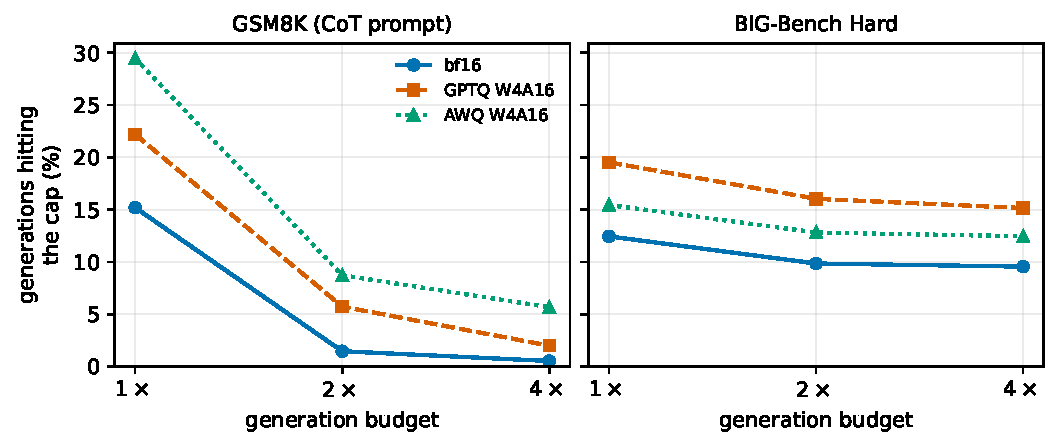
\includegraphics[width=\columnwidth]{../artifacts/figures/h1_cap_hit_rate}
\caption{Generations stopped by the budget rather than by the model, at three budgets.}
\label{fig:h1}
\end{figure}

\emph{Quantization shifts whether the model answers at all.} Against \texttt{bf16} on the same
items, \hFourExcludesNull{} of \hFourEffects{} per-cell comparisons change commitment
significantly, in both directions. For \hFourChurnArm{} on \hFourChurnTask{},
\hFourChurnLost{} items lose a committed answer and \hFourChurnGained{} gain one, a net of
only \hFourChurnNet~pp. This explains the negative interactions of \S\ref{sec:h3}: where a
quantized arm already commits more often, leniency has less left to recover.

\emph{Even a single-letter answer space does not protect the delta.} On ARC-Challenge we scored
the same \hSixItems{} items both by generation and by the log-likelihood of the four letters,
which removes extraction. On Phi-3.5 and Llama-3.1 the difference between the two quantization
deltas is at most \hSixMaxOther{}~points. On Qwen2.5 it is \hSixQwenGptq{}~points for GPTQ
(95\% CI \hSixQwenGptqCI{}) and \hSixQwenAwq{} for AWQ, the only \hSixRejected{} of \hSixM{}
contrasts that survive correction. Qwen's \texttt{bf16} model often answers in prose and is
cut off before a letter appears, so under generation it scores \hSixQwenBfGen\% against
GPTQ's \hSixQwenGptqGen\%, while under log-likelihood they score \hSixQwenBfLL\% and
\hSixQwenGptqLL\%: the sign of the delta reverses.

\section{Discussion}
\label{sec:discussion}

\emph{Pin two factors and report the third.} Item ordering and the process boundary are
nuisance parameters, so the remedy is to pin them. Generating every compared precision inside
one process removes the cross-process variation at no cost. Disabling the quantized kernels
removes the ordering variation for GPTQ and AWQ at about $3.7\times$ evaluation wall clock,
and does nothing for NF4. The extraction rule is a choice about what counts as correct, and its
effect varies by method and task, so it cannot be standardised away and has to be reported.

\emph{Recommend the test, not the flag.} A kernel flag is specific to one engine version. The
durable advice is a test: run the same items in several orderings and check that the outputs
agree bitwise, for whichever kernels your backend selected. We release that probe. A protocol
should also report the item submission order, whether compared precisions were generated in
one process, and the generation budget with its truncation rate.

\emph{Audit your own instrument.} The largest single error we found was ours: the extractor
defect of \S\ref{sec:method} changed two conclusions while every unit test passed, because no
fixture continued past its committed answer. A census over every item found it where a fixture
set could not, which is the same phenomenon this paper measures, seen from the inside.

\emph{Limitations.} All measurements use one engine version, so no result should be read as a
claim about other versions; the ordering result holds on two GPU architectures, and the
cross-process result was measured on one, with its cause undiagnosed. Three models support no
claim about a model population, and every task is a reasoning task with a regular-expression
extractor. The competence decomposition rests largely on bounds, because the always-compliant
stratum falls below half the paired items in \hFourStratumBelowHalf{} of \hFourStratumCells{}
cells. A stock AWQ checkpoint cannot be served in \texttt{bfloat16} on this engine version at
all, so published AWQ numbers are not dtype-comparable to GPTQ unless dtype is reported. Two
registered hypotheses, the trace-without-answer rate and the zero-shot interaction, are not
reported, because only partial numbers exist; they remain in the pre-registration.

\section{Conclusion}
\label{sec:conclusion}

Two unreported properties of an evaluation move reported quantization degradation, and both
are established by intervention or by a pre-registered contrast. Item submission order changes
4-bit accuracy while leaving \texttt{bf16} exactly unchanged, through quantized kernels that the
engine's batch-invariant mode does not cover. The extraction rule interacts with precision with
a sign that depends on the task and method, so it has to be reported rather than corrected
for. We release the full generation corpus so that any extraction rule can be re-evaluated
without a GPU.

\section*{Ethics and Data Statement}
We evaluate existing open-weight models on public benchmarks and introduce no new model and no
deployment. Every model and dataset is used within its licence: Qwen2.5-3B-Instruct is under the
Qwen research licence rather than Apache-2.0, and the judge's weights (CC-BY-NC-ND-4.0) are run
but never redistributed. Human labels come from two annotators following a written rubric, with
the precision condition and every automated verdict withheld from the annotation file. Our
results concern the \emph{difference} between arms under a fixed protocol, not whether
quantization is safe to deploy, and should not be read as licence to dismiss reported
degradation. The corpus, the probe, the rubric and labels, and a log of every run (about 44
GPU-hours on single-GPU instances) are released.

\bibliographystyle{IEEEtranN}
\bibliography{../paper/custom}

\end{document}
